Para aplicar o método PCA, precisamos importá-lo da biblioteca \verb|sklearn|. Para visualização da quantidade de variáveis que explicam pelo menos 90\% da variância dos dados, podemos importar a biblioteca \verb|matplotlib|.
\begin{longlisting}
    \begin{minted}{py}
        import matplotlib.pyplot as plt
        from sklearn.decomposition import PCA
    \end{minted}
\end{longlisting}

Feito isso, somos capazes de aplicar a redução de variáveis pelo método PCA. Primeiro criamos uma instância do PCA, em seguida ajustamos o modelo PCA aos dados de \verb|X|, calculando as componentes principais com suas variâncias e por fim transformas os dados originais de \verb|X| para o espaço das componentes principais (\verb|x|).
\begin{longlisting}
    \begin{minted}{py}
        pca = PCA()
        pca.fit(X)
        x = pca.transform(X)
    \end{minted}
\end{longlisting}

Feita a transformação dos dados, podemos determinar a quantidade de variáveis que vão determinar ao menos 90\% da variância dos dados. Começamos obtendo a proporção de variância explicada por cada componente principal, seguindo da soma cumulativa destas proporções (explicabilidade). Com isso podemos encontrar o número de componentes necessárias para atingir mais de 90\% da variância
\begin{longlisting}
    \begin{minted}{py}
        propVarExpl = pca.explained_variance_ratio_
        explainability = propVarExpl.cumsum()
        factors = np.arange(1, x.shape[1] + 1, 1)
        p = factors[explainability < 0.9].max() + 1
        if p < 2:
            p = 2
        
        print(f"90% dos dados são explicados por {str(p)} componentes")
    \end{minted}
\end{longlisting}
cujo output retorna a resposta: 
\begin{verbatim}
    90% dos dados são explicados por 4 componentes
\end{verbatim}

Que podemos ver graficamente
\begin{longlisting}
    \begin{minted}{py}
        plt.scatter(factors, explainability)
        plt.hlines(0.9, 0, 12,'r', linestyle = '--')
        plt.xlabel('Número de componentes');
        plt.ylabel('Explicabilidade dos dados');
    \end{minted}
\end{longlisting}
\begin{figure}[H]
    \centering
    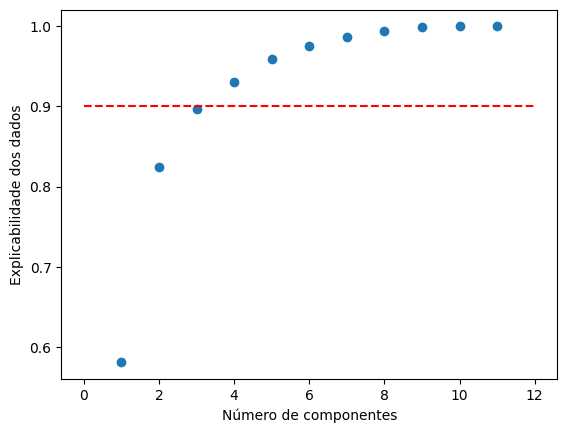
\includegraphics[width=0.6\linewidth]{figures/explicability2.png}
\end{figure}

% Por fim, sabendo a quantidade de variáveis necessárias para descrever pelo menos 90\% da variância dos dados, podemos reduzir a dimensionalidade de \verb|X| para apenas \verb|p = 4| componentes e guardar em \verb|x|.
% \begin{longlisting}
%     \begin{minted}{py}
%         pca = PCA(n_components = p)
%         pca.fit(X)
%         x = pca.transform(X)
%     \end{minted}
% \end{longlisting}